\documentclass[spanish, c]{beamer}

\usepackage[utf8]{inputenc}
%\usepackage[spanish, mexico]{babel}
\usepackage{amsmath}
\usepackage{mathtools}
\usepackage{hyperref}
\usepackage{xcolor}
\usepackage{color}
\usepackage{ragged2e}
\usepackage{mathrsfs}
\usepackage{csquotes}
\usepackage{listings}
\usepackage[scaled]{beramono}
\usepackage[T1]{fontenc}
\usepackage{matlab-prettifier}
\usepackage{graphicx}
\usepackage{booktabs}
\usepackage{physics}

\renewcommand{\indent}{\hspace*{2em}}

% \usepackage{tikz}

% \usetikzlibrary{fit, shapes, arrows}

% \usepackage{courier}
% \usepackage{subfigure}
% \usepackage{enumerate}
% \usepackage{algorithmic}
% \usepackage{algorithm}

% \usepackage{listings}
% \usepackage{lstlinebgrd}

\usetheme{Boadilla}
\usefonttheme[onlymath]{serif}

\newcommand{\matlab}[1]{\lstinline[style=Matlab-editor]!#1!}
\newcommand\blfootnote[1]{%
\begingroup
\renewcommand\thefootnote{}\footnote{#1}%
\addtocounter{footnote}{-1}%
\endgroup
}

\lstset
{
    language = Matlab,
    style = Matlab-editor,
    basicstyle = \mlttfamily\scriptsize,
    escapechar = `,
    numbers = left,
    frame = tb,
}

\lstdefinestyle{output}
{
    language = {},
    basicstyle = \mlttfamily\scriptsize,
    escapechar = `,
    numbers = none,
    showtabs = false,
   	showstringspaces = false,
}

% Sets the templates
\definecolor{navyblue}{RGB}{0, 0, 128}
\definecolor{crimson}{RGB}{128, 16, 0}

\setbeamertemplate{navigation symbols}{}
\setbeamertemplate{headline}{}
\setbeamertemplate{title page}[default][colsep=-4bp,rounded=true]
\setbeamertemplate{footline}[frame number]
\setbeamertemplate{bibliography item}[text]
\setbeamertemplate{theorems}[numbered]

\setbeamercolor{title}{fg=navyblue, bg=white}
\setbeamercolor{frametitle}{fg=navyblue, bg=white}
\setbeamercolor{structure}{fg=navyblue}
\setbeamercolor{button}{fg=white,bg=navyblue}

\setbeamercovered{transparent}

\title{Raíces: \textit{Bracketing Methods}}
\subtitle{Aplicación de Métodos Numéricos al Ambiente Construido \\ (CV1012)}
\author{
    \texorpdfstring{
        \begin{center}
            M.C. Xavier Sánchez Díaz \\
            \href{mailto:sax@tec.mx}{\texttt{sax@tec.mx}}
        \end{center}
    }
    {M.C. Xavier Sánchez Díaz}
}

\institute[Tecnológico de Monterrey]{
\includegraphics[scale=0.5]{../img/logo}}
\date{}

\begin{document}

\setlength{\rightskip}{0pt}

\begin{frame}[plain]
    \titlepage        
\end{frame}

\begin{frame}{Outline}
    \tableofcontents
\end{frame}

\section{Raíces}

\begin{frame}{¿Qué es una raíz?}{Raíces}

    \begin{block}{Definición}
        La raíz de una función $f$ (también llamada \textit{cero}) es un número $x$ tal que $f(x) = 0$.    
    \end{block} \pause

    \bigskip

    En otras palabras, la raíz de una función hace referencia al \alert{valor numérico} de una \textbf{variable independiente} cuando la \textbf{variable dependiente} vale 0. \pause

    \bigskip

    En palabras aún más simples, una raíz se puede identificar \textbf{gráficamente} como el punto donde la gráfica de una función corta al eje de las $x$.

\end{frame}

\begin{frame}{¿Para qué me sirve encontrar una raíz?}{Raíces}

    ¿Qué significa cada raíz en esta gráfica si $f(x)$ fuera velocidad? ¿Qué valores tienen?

    \begin{center}
        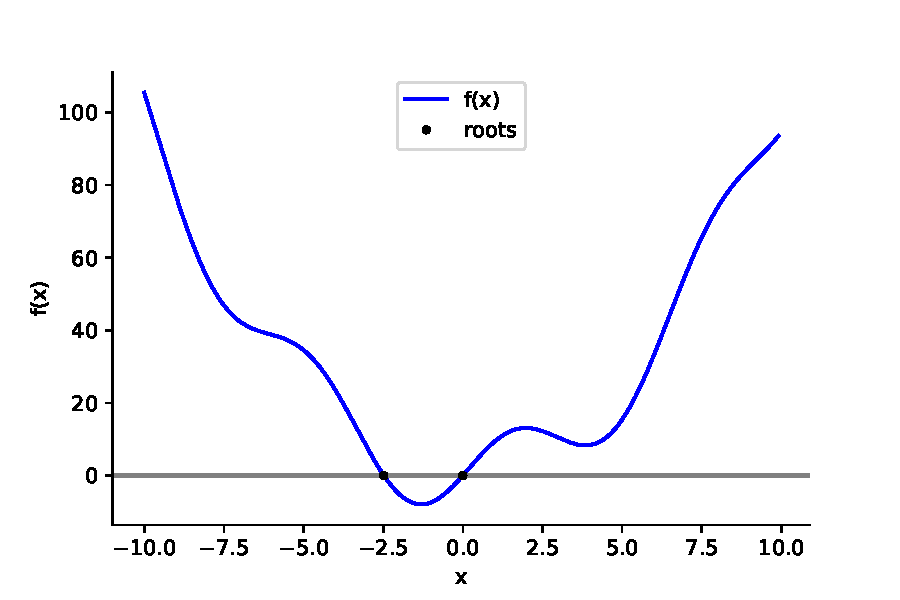
\includegraphics[width=0.75\textwidth]{roots.pdf}
    \end{center}

\end{frame}

\begin{frame}{Bisección}{Método de bisección}

Sabiendo que nuestra función es $f(x) = x^2 + 10 \sin(x)$, intentemos encontrar \textbf{gráficamente} la raíz exacta que está cerca del -$2.5$. \pause

\bigskip

Primero, delimitemos puntos de \textit{más o menos} dónde podría estar: \pause

\begin{itemize}
    \item Uno de ellos tendría que ser donde la evaluación de $f(x)$ dé como resultado un número positivo---es decir, por \textbf{arriba} del 0. \pause
    \item El otro por \textbf{debajo} del 0.
\end{itemize} \pause

\bigskip

Para este caso, pensemos en $-3$ y $-2$, donde

$$f(-3) = 7.588799919 \quad \text{ y } \quad f(-2) = -5.092974268$$

\end{frame}

\begin{frame}{Bisección}{Método de bisección}
    Encontremos el punto medio entre nuestros dos límites con un simple promedio:
    $$x_r = \frac{-3 + (-2)}{2} = -2.5$$ \pause
    \bigskip
    Y ahora evaluemos la función en la aproximación: $f(-2.5) = 0.26528$. \pause
    \bigskip
    Con este nuevo número, ahora revisemos cuánto da la multiplicación de las evaluaciones de este nuevo punto y del límite inferior:
    $$f(-3) \cdot f(-2.5) = (7.588799919)(0.26528) = 2.0131$$ \pause
    Y como este número es positivo, significa que no ocurrió un cambio de signo\footnote{¿Por qué podemos asumir esto?}.
\end{frame}

\begin{frame}{Bisección}{Método de bisección}
    Este proceso es conocido como el \alert{método de bisección}.
    Repetimos el procedimiento:

    \begin{enumerate}[<+->]
        \item Bisectamos: $x_r = \frac{-2.5 + (-2)}{2} = -2.25$
        \item Evaluamos: $f(-2.25) = -2.7182$
        \item Probamos con límite inferior: $f(-2.5) \cdot f(-2.25) = (0.26528)(-2.7182) = -0.72109$
        \item Revisamos el signo del paso 3. Si es positivo, entonces probamos con el otro límite. Si es negativo, entonces usamos $x_r$ como nuevo límite.
        \item Medimos el error: $\varepsilon_a = \frac{-2.5 - (-2.25)}{-2.5} = 0.1$
    \end{enumerate} \pause
    
    Y seguiremos repitiendo, hasta que $\varepsilon_a$ sea lo suficientemente pequeño.
\end{frame}

\section{Falsa posición}

\begin{frame}{Convergencia}{Falsa Posición}
    Cuando hablamos de \alert{convergencia}, nos referimos al \textbf{momento} en el que se encuentra una \textit{solución aceptable}. \pause
    
    \bigskip

    ¿Qué tan \textit{rápido} converge el método de la bisección? Pensemos en intervalos de `mitades' \pause

    \bigskip

    \begin{enumerate}[<+->]
        \item El punto medio entre -2 y -3 es \textbf{-2.5}
        \item El punto medio entre -2 y -2.5 es \textbf{-2.25}
        \item El punto medio entre -2.25 y -2.5 es \textbf{-2.375}
        \item El punto medio entre -2.375 y -2.5 es \textbf{-2.4375}
        \item El punto medio entre -2.4375 y -2.5 es \textbf{-2.46875}
        \item El punto medio entre -2.46875 y -2.5 es \textbf{-2.484375}
        \item \dots
    \end{enumerate} \pause

    ¿Cuánto hay entre los resultados del paso 1 y el 2? \pause ¿Y entre el 2 y el 3? ¿Y entre el 3 y el 4?
\end{frame}

\begin{frame}{Convergencia}{Falsa posición}
    \begin{center}
        {\huge ¿Podemos hacer que converja más rápido?}
        (\textit{Spoiler alert: sí podemos.})
    \end{center}
\end{frame}

\begin{frame}{El método de la falsa posición}{Falsa posición}

    El método de la \alert{falsa posición} consiste en generar una \textit{raíz falsa}, más cerca de la verdadera raíz que alguno de los dos límites que usamos en el método de bisección. \pause

    \bigskip

    Usando una línea recta podemos deducir dónde estará nuestra \textbf{falsa posición} y luego trabajar con eso:

    $$ x_r = x_u - \frac{f(x_u)(x_l - x_u)}{f(x_l) - f(x_u)}$$ \pause

    Usando los mismos pasos del algoritmo de bisección, lo único que incorporaremos para mejorar el algoritmo es cambiar el paso de bisección por este nuevo paso y listo.

\end{frame}

\section{Notas sobre los \textit{bracketing methods}}

\begin{frame}{Notas sobre los \textit{bracketing methods}}

    \begin{itemize}
        \itemsep3ex
        \item Tanto el método de la falsa posición como el de la bisección se conocen como \textbf{métodos de intervalos} o en inglés, \textit{bracketing methods}.
        \item El método de la \textbf{falsa posición} no siempre es más rápido que el de bisección.
        \item El tamaño de los \textit{`brincos'} importa:
    \end{itemize}

    \begin{center}
        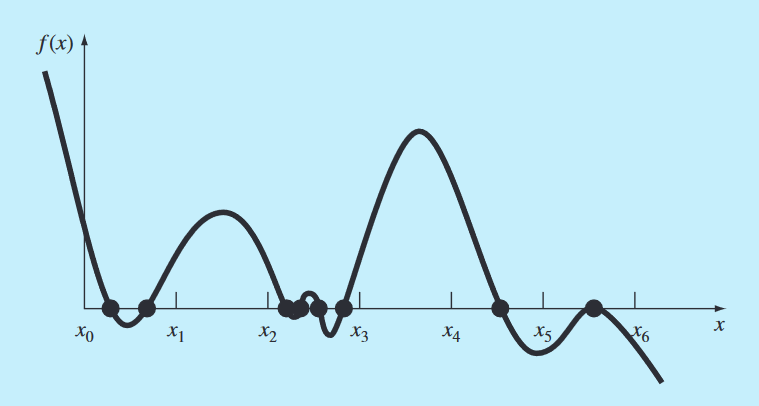
\includegraphics[width=0.5\textwidth]{steps.png}
    \end{center}

\end{frame}

% What is control flow
% why is it important
% does it exist in math?
% how to represent it
% how to represent it in matlab
% practical cases

% \section*{Referencias}

% \begin{frame}[t]{Referencias}
    % \nocite{bibID01}
    % \nocite{bibID02}

    % \bibliographystyle{IEEE}
    % \bibliography{biblio}
% \end{frame}

\end{document}